\documentclass[12pt]{article}
 
\usepackage[margin=1in]{geometry} 
\usepackage{amsmath,amsthm,amssymb}
\usepackage{hyperref}
\usepackage{graphicx}
\usepackage{xcolor}
\usepackage[many]{tcolorbox}
\tcbuselibrary{listings}
\usepackage{listings}

\definecolor{lg}{HTML}{f0f0f0}

\newtcblisting{pycode}{
    colback=lg,
    boxrule=0pt,
    arc=0pt,
    outer arc=0pt,
    top=0pt,
    bottom=0pt,
    colframe=white,
    listing only,
    left=15.5pt,
    enhanced,
    listing options={
        basicstyle=\small\ttfamily,
        keywordstyle=\color{blue},
        language=Python,
        showstringspaces=false,
        tabsize=2,
        numbers=left,
        breaklines=true
    },
    overlay={
        \fill[gray!30]
        ([xshift=-3pt]frame.south west)
        rectangle
        ([xshift=11.5pt]frame.north west);
    }
}

\lstset{
    language=Python,
    basicstyle=\small\ttfamily,
}

 
\begin{document}
 
\title{Exercise 3}
\author{Cristian Manuel Abrante Dorta - 888248\\
ELEC-E8125 - Reinforcement Learning}

\maketitle
\section{Cartpole}

\subsection{Task 1: Implement Q-learning for the Cartpole environment. Compare using a constant value of $\epsilon$ = 0.2 to reduce the value of $\epsilon$ over time}

The comparison of the results between the two versions of the Q-learning algorithm (for different values of $\epsilon$) was done by observing the plot of the average timesteps that the execution achieved, and also by observing the execution of the cartpole with the trained model.

\subsubsection{$\epsilon$ fixed to 0.2}

Running the Q learning algorithm for the fixed value of $\epsilon=0.2$ for 20000 episodes, gave as a result the following plot of the average timesteps length:

\begin{figure}[h]
    \centering
    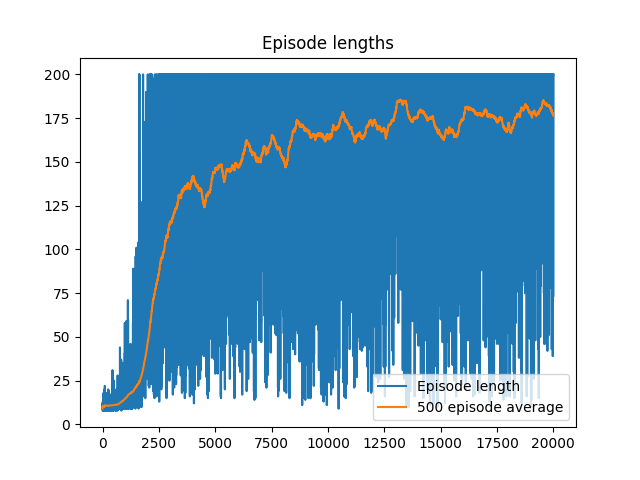
\includegraphics[scale=0.6]{exercise-3/plots/episodes-fixed-0.2.png}
    \caption{Average timesteps for the Q-Learning algorithm}
    \label{fig:fixed-0.2}
\end{figure}

In figure \ref{fig:fixed-0.2} is shown the evolution of the timesteps that the model is able to achieve over the training episodes. Variance is really significant over the executions, but the average tendency is to increase, reaching almost an stabilization level from episode 15000.\\

\subsubsection{GLIE $\epsilon$}

For the \textit{greedy in limit with infinite exploration} technique, the $\epsilon$ variable was setted according to this formula:

\begin{equation}
    \epsilon = \frac{a}{a + p}
\end{equation}

Where each variable meant:

\begin{itemize}
    \item $p$: Current episode of the training execution.
    \item $a$: This is the constant integer variable used for the decrement of the epsilon over the training episodes. The value was established in a way that in the final execution, the $\epsilon$ variable will be 0.1:
    \begin{equation}
        a = \frac{\epsilon}{1 - \epsilon}p; \quad \quad a = \frac{0.1}{1-0.1}\cdot20000; \quad \quad a = 2222
    \end{equation}
\end{itemize}

Having this formula specified, we can execute the training, observing the corresponding plot for the average timesteps:

\begin{figure}[h]
    \centering
    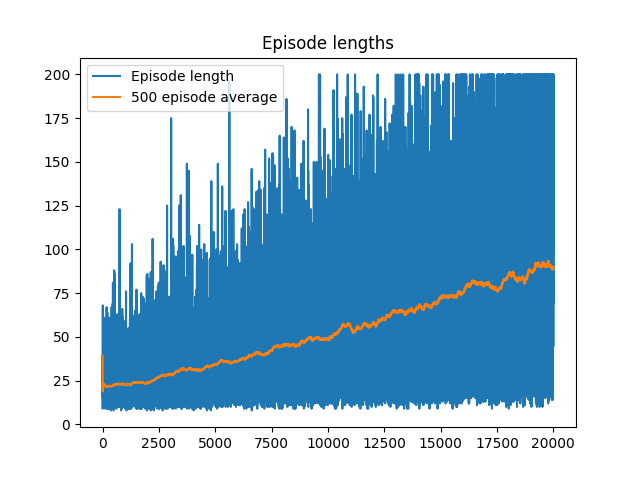
\includegraphics[scale=0.6]{exercise-3/plots/episodes-variable-0.0.png}
    \caption{Average timesteps for the Q-Learning algorithm}
    \label{fig:variable}
\end{figure}

As we can see in figure \ref{fig:variable}, the tendency of the average timesteps is to increase over the episodes, performing slightly better compared to the fixed value of $\epsilon$ (Figure \ref{fig:fixed-0.2}). \\

As there is only an small difference between the performance of both algorithms (even though the GLIE is better), both of the executions in the cartpole environment lead to successful results, having an agent wich is capable of balancing the pole all over the timesteps.

\subsection{Task 2: Plot the optimal value function of each state}

After the execution of the training for both types of algorithms, we can plot the optimal value for each state:

\begin{figure}[ht]
    \centering
   \begin{minipage}{0.48\textwidth}
     \centering
     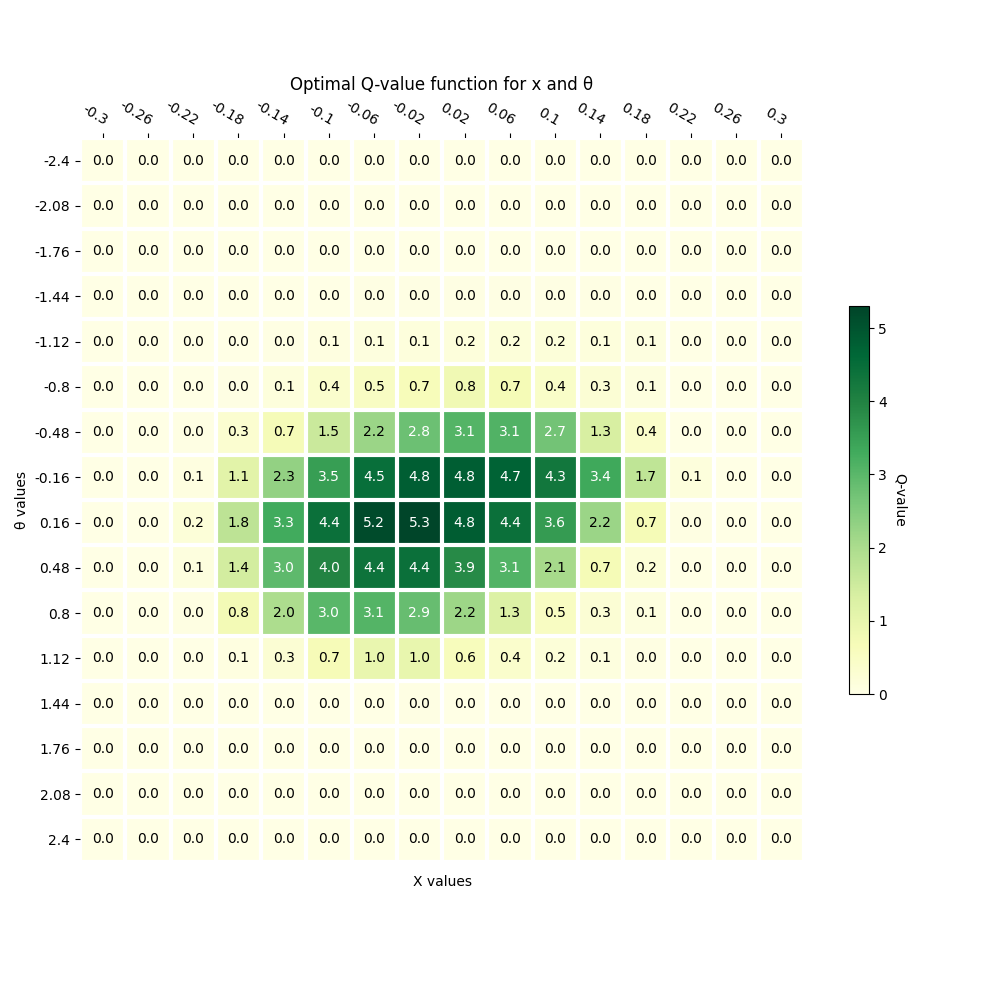
\includegraphics[width=0.9\linewidth]{exercise-3/plots/heatmap-fixed-0.2.png}
     \caption{Heatmap of the optimal Q-value for $\epsilon=0.2$}
     \label{fig:task-2-1}
   \end{minipage}\hfill
   \begin{minipage}{0.48\textwidth}
     \centering
     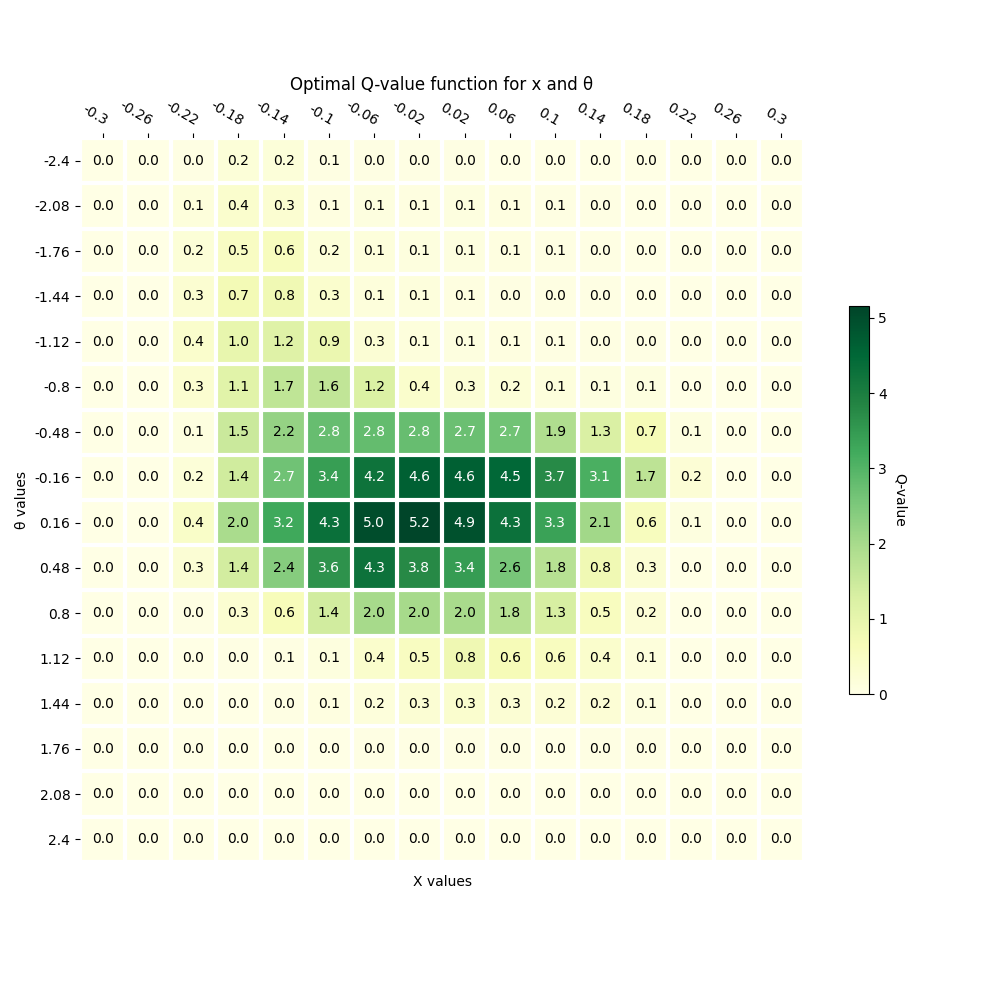
\includegraphics[width=0.9\linewidth]{exercise-3/plots/heatmap-variable-0.0.png}
     \caption{Heatmap of the optimal Q-value for variable $\epsilon$}
     \label{fig:task-2-2}
   \end{minipage}
\end{figure}

In those plots the difference between both algorithms is well seen. In the $\epsilon$-fixed version (Figure \ref{fig:task-2-1}), we can see that the exploration of the state space is limited, because the agent is greedy more frequently.\\

On the variable $\epsilon$ version (Figure \ref{fig:task-2-2}), we can notice that even tough there is a concentration in the selected actions, the state space has more states explored. This is because in the initial phases of the training the $\epsilon$ value have a high value, so random actions are selected in many situations.

\section{Task 2}
To embed code snippets in the report, you can use the \texttt{pycode} environment.

\begin{pycode}
for episode_number in range(train_episodes):
    reward_sum, timesteps = 0, 0
    done = False
    # Reset the environment and observe the initial state
    observation = env.reset()

    # Loop until the episode is over
    while not done:
        # Get action from the agent
        action, action_probabilities = agent.get_action(observation)
        previous_observation = observation

        # Perform the action on the environment, get new state and reward
        observation, reward, done, info = env.step(action)

        # Store action's outcome (so that the agent can improve its policy)
        agent.store_outcome(previous_observation, action_probabilities, action, reward)

        # Draw the frame, if desired
        if render:
            env.render()
\end{pycode}

\section{Question 1}

If you add a figure, you can refer to it using Figure.~\ref*{fig:fig1}.

\begin{figure}[h] 
	\centering  % Remember to centre the figure
    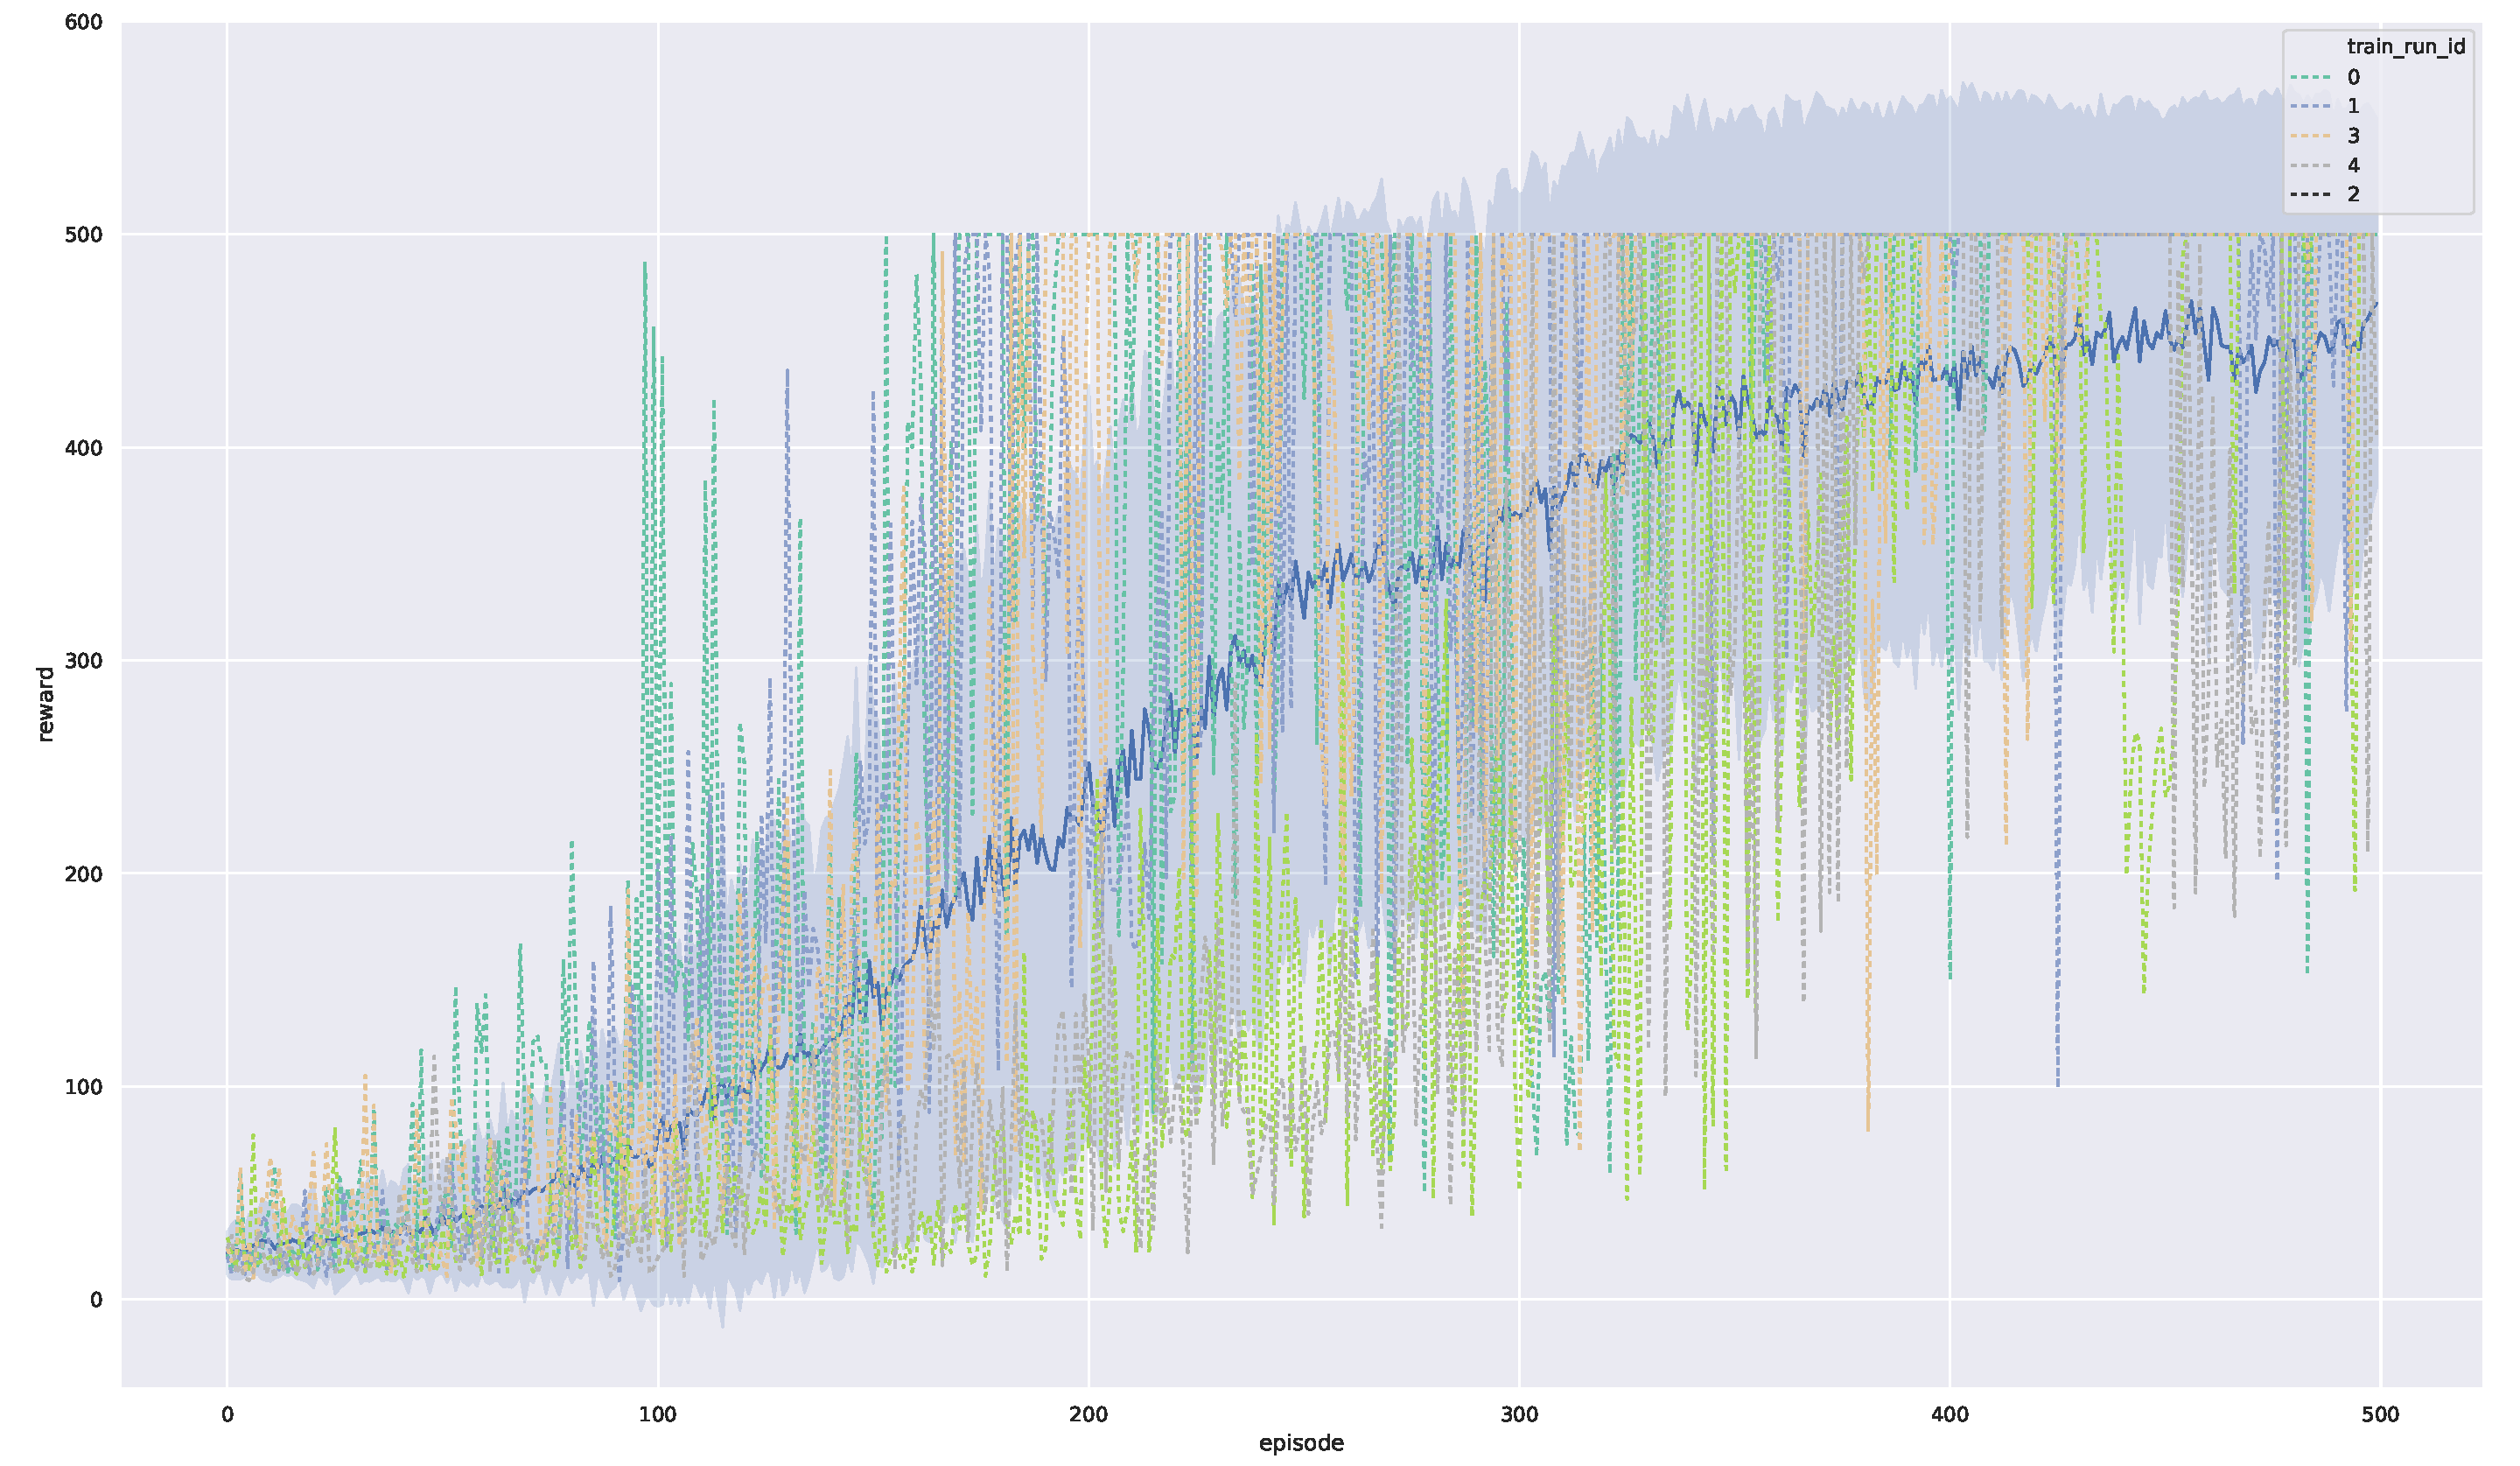
\includegraphics[width=0.9\columnwidth]{img/training.pdf}
	\caption{This is a sample figure.}
	\label{fig:fig1}
\end{figure}

\bibliographystyle{ieeetr}
\bibliography{bibliography}  % Modify template with your bibliography name
\end{document}
